\let\negmedspace\undefined
\let\negthickspace\undefined
\documentclass[journal]{IEEEtran}
\usepackage[a5paper, margin=10mm, onecolumn]{geometry}
%\usepackage{lmodern} % Ensure lmodern is loaded for pdflatex
\usepackage{tfrupee} % Include tfrupee package

\setlength{\headheight}{1cm} % Set the height of the header box
\setlength{\headsep}{0mm}     % Set the distance between the header box and the top of the text

\usepackage{gvv-book}
\usepackage{gvv}
\usepackage{cite}
\usepackage{amsmath,amssymb,amsfonts,amsthm}
\usepackage{algorithmic}
\usepackage{graphicx}
\usepackage{textcomp}
\usepackage{xcolor}
\usepackage{txfonts}
\usepackage{listings}
\usepackage{enumitem}
\usepackage{mathtools}
\usepackage{gensymb}
\usepackage{comment}
\usepackage[breaklinks=true]{hyperref}
\usepackage{tkz-euclide} 
\usepackage{listings}
% \usepackage{gvv}                                        
\def\inputGnumericTable{}                                 
\usepackage[latin1]{inputenc}                                
\usepackage{color}                                            
\usepackage{array}                                            
\usepackage{longtable}                                       
\usepackage{calc}  
\usepackage{amsmath,amssymb}

\usepackage{multicol}                                         
\usepackage{hhline}                                           
\usepackage{ifthen}                                           
\usepackage{lscape}
\begin{document}

\bibliographystyle{IEEEtran}

\title{
%	\logo{
NCERT - 11.16.1.3

\large{EE1003}
%	}
}
\author{Homa Harshitha Vuddanti

(EE24BTECH11062)
}	

\maketitle

\bigskip

\renewcommand{\thefigure}{\theenumi}
\renewcommand{\thetable}{\theenumi}
\textbf{Question}: Find the PMF of the binomial random variable for the experiment - A coin is tossed four times.
\textbf{Solution: }\\
Let $X$ be the number of heads in four independent tosses of the fair coin.\\
\begin{align}
    X=X_1+X_2+X_3+X_4
\end{align}
Let $X_i$ be the Bernoulli random variable.\\
$X$ is the Binomial random variable.\\
\begin{align}
X_i=
\begin{cases}
	1, & \text{outcome is Heads}\\
	0, & \text{outcome is Tails}
\end{cases}
\end{align}
\textbf{Compute the moment generating function \brak{MGF} using the $\mathcal{Z}$-transform:}\\
The $\mathcal{Z}$-transform of the PMF is given by
\begin{align}
      M_{X_i}(z) &= \sum_{n=-\infty}^{\infty} p_{X_i}(n) z^{-n}
\end{align}
 Since $X_i$ takes only two values (0 or 1):
    \begin{align}
        M_{X_i}(z) &= (1-p)+pz^{-1}\
    \end{align}
    \text{since} $X_1,X_2,X_3,X_4$\text{are independent, their total MGF is:}
    \begin{align}
        M_X(z) &= M_{X_1}(z)M_{X_2}(z)M_{X_3}(z)M_{X_4}(z)\\
        M_X(z) &= ((1-p)+pz^{-1})^4\\
        M_X(z) &= \sum_{n=-\infty}^{\infty}\comb{4}{n}(1-p)^{4-n}p^nz^{-n}\\
	p_{X}(n) &= \comb{4}{n}p^{n}(1-p)^{4-n}
\end{align}
Sunstituting $p=\frac{1}{2}$
\begin{align}
	p_{X}(n) &= \frac{\comb{4}{n}}{16}
    \end{align}
    The Probability Mass Function (PMF) for the given random variable is
\begin{align}
p_X(n) =
\begin{cases}
	\frac{1}{16}, & n = 0 \\
	\frac{1}{4}, & n = 1 \\
	\frac{3}{8}, & n = 2 \\
	\frac{1}{4}, & n = 3 \\
        \frac{1}{16}, & n=4\\
\end{cases}
\end{align}
\textbf{Plotting:}\\
We generate random numbers between $0$ and $1$, and classify them as heads if it is less than 0.5 and tails if it is greater than 0.5. We repeat this trial 4 times to get number of heads in an experiment. This is repeated large number of times and number of heads at k=0,1,2,3,4 is divided with number of trials to get probability.
\begin{figure}[h!]
   \centering
   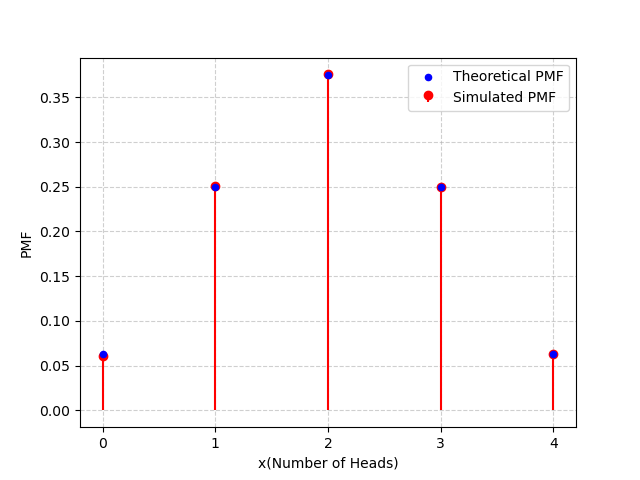
\includegraphics[width=1\columnwidth]{Figs/Figure_1.png}
   \caption{Plot}
\end{figure}
\end{document}






